\documentclass[14pt, landscape]{article}

\usepackage{common}
\pagenumbering{gobble}

\begin{document}

\begin{center}
	{\fontfamily{qag}\fontsize{16}{12}\selectfont Variational Autoencoders}
\end{center}

\vspace{10mm}

\begin{figure}[h!]
	\centering
	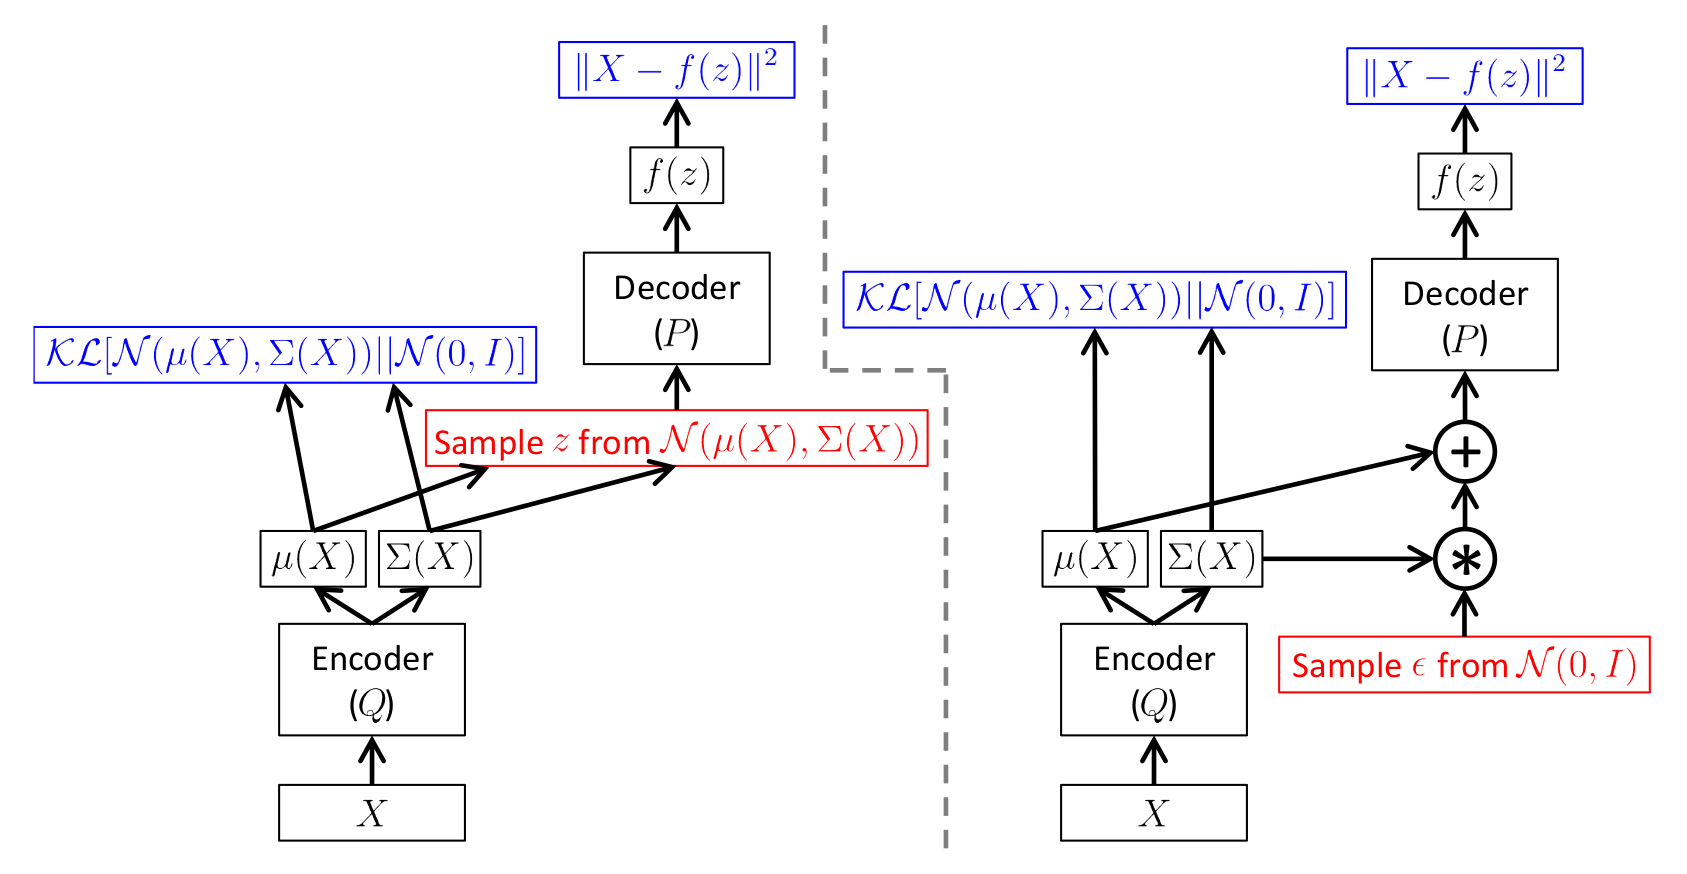
\includegraphics[width=0.8\textwidth]{vae.png}
	\caption{A basic example of a VAE}
\end{figure}

\bt{\fontfamily{qag}\fontsize{13}{12}\selectfont Optimization Terms}

{\fontsize{13}{12}\selectfont
	\begin{align*}
		&&\mdef{KL Loss} \quad\quad	\text{KL}\brac{\ND{\vmu(X), \Sigma(X)} \pipe \ND{\vzero, \vI}}	&\eq	\frac{1}{2} \para{\trace{\Sigma(X)} + \tr{\para{\vmu(X)}} \para{\vmu(X)} - D + \log{\tfunc{det}{\Sigma(X)}}}& \\
		\\
		&&\mdef{Reconstruction Loss} L	&\eq	\norm{X - z}_2^2 &
	\end{align*}
}
\end{document}
